\chapter{Escalation to Human Experts}\label{chap:escalation}

The techniques presented in the previous chapters allow WCA applications to
detect states that the developer trains models to handle.
The developer can provide example images of the object after each step has been
done correctly.
However, there are many possible ways that an object can be put together
incorrectly.
It is not possible to collect images of every mistake that someone completing a
task might make.
People using these
applications in the real world are going to reach some states that the models
were not trained for. As Dr. Reynold Xin once said,
``A machine learning model is only as good as the data it is fed~\cite{xin}.''
Our models can signal to our application that an image ``looks most similar to
this set of images from the training data.''
These models are not capable of a more general understanding, such as ``the long
brass piece is screwed on upside down.''

Detecting all possible error states would require us to have examples of these
states in our training data. There is a combinatorial explosion in the number of
error states, compared to the number of correct states, so collecting training
data for every possible error is not practical.
Instead, we handle errors that our models were not trained to recognize by
having people completing tasks call a human expert from the application.
The user's camera feed during these calls can be recorded, and these recordings
can provide data to train models to recognize these errors in the future.
This allows us to follow a DevOps strategy when developing these applications.
A team of developers can launch an initial version of a WCA application that
detects a small number of error states.
As the application gets used, and people call in to get help with new errors,
the developers can improve the application to detect these errors.
Over time, this process will increase the number of error states that our
application can detect.

\section{Experts Without Automation}

Several commercial products allow a remote human expert to help a user through
an assembly task.
Examples of such systems include Microsoft Dynamics 365 Remote
Assist~\cite{dynamics365}, Webex Expert on Demand~\cite{webex},
AMA XpertEye~\cite{xpert}, and Vieaura~\cite{vieaura}.
The person completing the task wears a headset with a camera, but the expert
must be on a call with a single user for the duration of an entire task.
A task expert's time is valuable.
We believe that integrating wearable cognitive assistance with
human assistance will allow products like these to scale from requiring
experts to work one on one through each step of the task to enabling experts to
help multiple users concurrently.

\section{Calls With Human Experts}

The computer vision models that our applications use are not perfect. In order
to handle cases where a model makes a mistake, our applications allow the user
to start a call with a human who is an expert on the task being completed. The
human expert sees a feed from the user's camera and they can talk the user
through correcting problems. In addition, the expert can change the step that
the application thinks the user is in the middle of, and then the user can
continue to receive guidance from the application after the call ends.
The application can also be modified to suggest calling the expert, if a user
has been stuck on a step for a certain amount of time.
However, additional research is required to determine what should trigger a
suggestion to call the expert.
Potential options include triggering a suggestion after the application has seen
a sequence of frames with identical perceptual hash
values, or simply a certain amount of time passing without the user advancing a
step.
In addition, it might not be necessary to suggest calling the expert in the
first place, as users have the option to start the call at any point.
Figure~\ref{fig:design_space} shows options for task guidance systems that use
human experts.

\begin{figure}[h]
  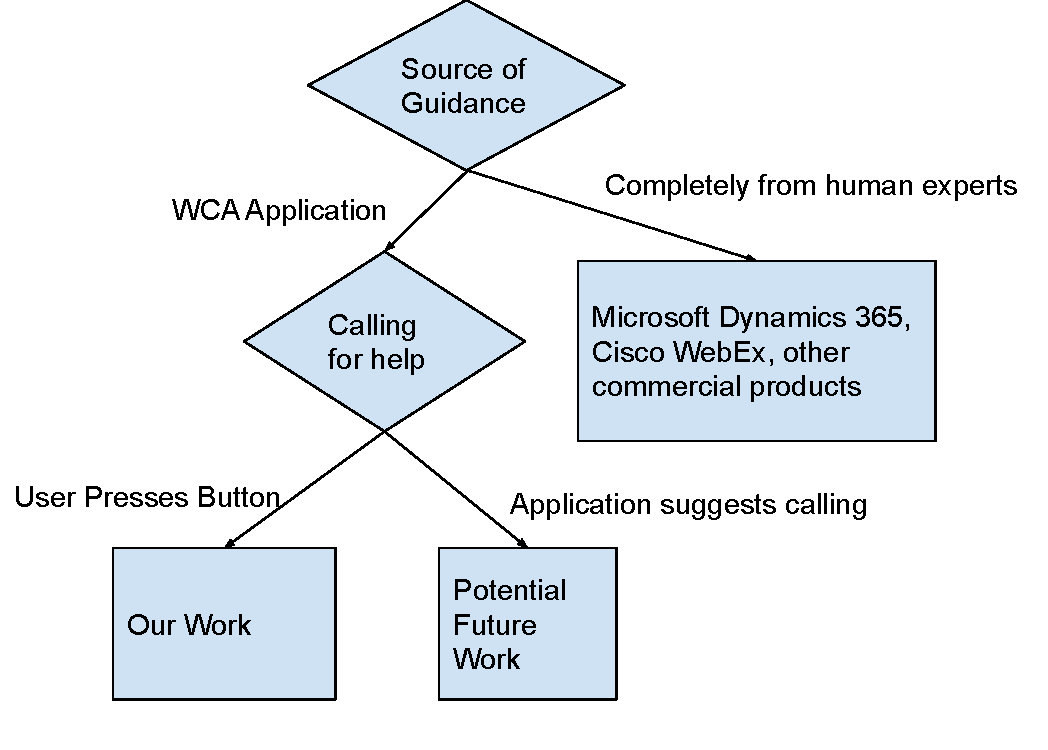
\includegraphics[width=10cm]{figures/design_space.pdf}
  \caption[
  The design space of remote expert assistance systems for assembly tasks
  ]{
    The design space of remote expert assistance systems for assembly tasks.
    Our system primarily guides users with a WCA application.
    Users must explicitly press a button to start a call with a human expert.
  }\label{fig:design_space}
\end{figure}

When we train models for Gabriel applications, we consider each state of a task
to be one object. Open World Object Detection~\cite{joseph2021open} is an active
area of research into models that can learn to detect previously unlabeled
objects. However, this does not help with recognizing such an object the first
time it is seen. Gabriel applications need to handle all errors, even ones that
have not been seen before. A human who is an expert on the task can do this.

Correcting error states in Gabriel applications can be done on the order of tens
of seconds to a few
minutes, unlike driving a car which might require sub-second response times.
It's perfectly acceptable for the user to press a button to call for help from
an expert, if the application does not detect that a step has been completed
after a certain amount of time. The user will then be connected to someone who
is an expert on this task. The expert will
see the camera feed from the headset and talk back and forth with the user to
help them get back to a state that the computer vision models can handle.
The expert will also have the ability to update the application's state, so the
user can continue receiving automated guidance from an earlier or later
step after the call.
This workflow is depicted in Figure~\ref{fig:zoom_workflow}.

\begin{figure}[h]
  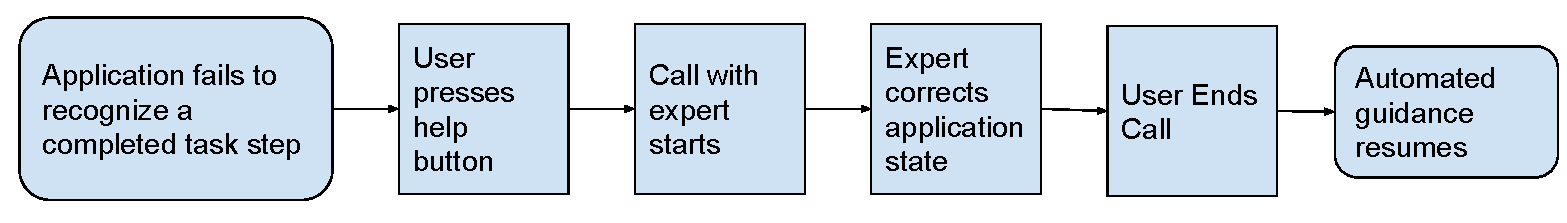
\includegraphics[width=\textwidth]{figures/zoom_workflow.pdf}
  \caption{
    The workflow followed to request help from a human expert
  }\label{fig:zoom_workflow}
\end{figure}

We connect users to task experts using Zoom, which offers SDKs for several
platforms~\cite{zoom}. The Gabriel user runs an Android application on a
smartphone or Google Glass, which starts a call with the expert using Zoom's
Android SDK.
The human expert uses a web application that incorporates Zoom's Web SDK.
The components of the system are shown in Figure~{\ref{fig:expert_components}}.
Figure~{\ref{fig:expertui}} shows a screenshot of the application used by the
human expert.
The expert's web application allows them to see the user's camera feed, as well
as the step that the user is currently working on.
The application works for any WCA task that was created with Open Workflow
Editor.
The code can be modified to use a different video calling service in the future.

\begin{figure}[h]
  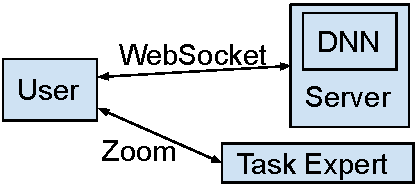
\includegraphics[width=8cm]{figures/human_assitance.pdf}
  \caption[The components of a Gabriel application with human assistance]{
    The components of a Gabriel application with human assistance.
    The user primarily receives guidance from a server running a DNN.
    If the user reaches a point where the automated assistance fails, they can
    switch over to receiving guidance from a human expert over a video call.
  }\label{fig:expert_components}
\end{figure}

\begin{figure}[h]
  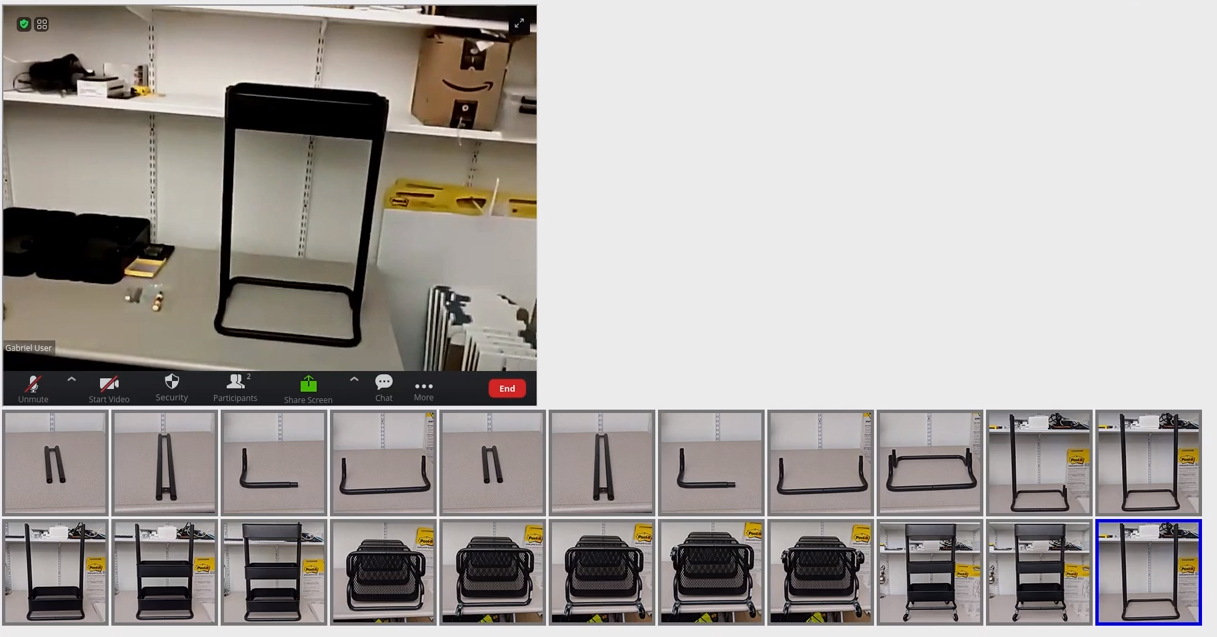
\includegraphics[width=\textwidth]{figures/expert_ui.png}
  \caption[A screenshot of the web application used by the human task expert]{
    A screenshot of the web application used by the human task expert.
    The feed from the user's camera is shown on top.
    The task steps are shown on the bottom.
    The step that the application believes the user is currently working on is
    surrounded by the blue box.
    Clicking on a different step will change the current step to the one that
    was clicked on.
  }\label{fig:expertui}
\end{figure}

\section{Simulating Call Centers}

Supporting a large number of people using WCA applications at the same time
would require multiple human experts answering support calls.
It is important to employ enough experts to ensure that wait times are
reasonable.
However, having too many experts working at one time will create unnecessary
expenses.

We developed a simulation that people running a call center for a WCA
application could use to determine the number of experts they should have
available to assist the users who call for help.

There is a large body of work examining wait times for call
centers~\cite{queue1, queue2}.
Our work is different because we simulate a user completing a task with a WCA
application.
A single user might call the expert multiple times, if they get stuck on
multiple steps.
In addition, we model user patience, to determine the amount of time a user will
wait before calling the expert.

\subsection{A Simple Model}\label{sec:simple}

Kendall's notation is used to describe queuing models, by specifying the arrival
process, the distribution of service times, and the number of
servers~\cite{kendall}.
The arrival process determines how the amount of time between calls to the
expert should be sampled.
The amount of time that a user and an expert spend on a call with each other is
the service time.
The number of servers refers to the number of experts.

M/M/N is an example of Kendall's notation, where the queue has a Poisson arrival
process, a Poisson service time distribution, and more than one server.
The time between events for a Poisson arrival process follows an exponential
distribution.
An exponential distribution has the probability density function
$\lambda * e ^ {- \lambda x}$ when x is above 0.
As shown in Figure~\ref{fig:simple_sim1_dists}, it takes the form of a
negatively accelerated decreasing function of x, where the rate of decrease is
governed by $\lambda$.

\begin{figure}[h]
  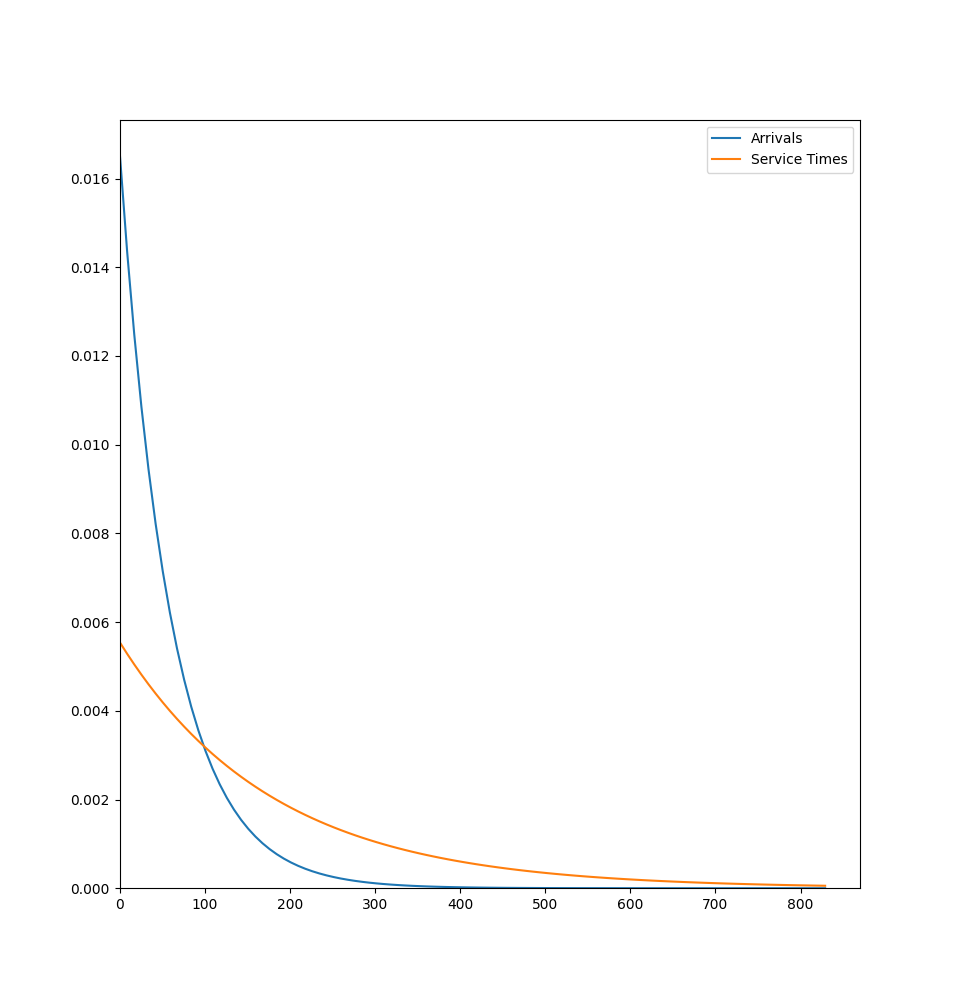
\includegraphics{figures/montecarlo/expon_expon.png}
  \caption[The PDFs for the distributions that Simulation 1 samples from]{
    The PDFs for the distributions that Simulation 1 samples from.
    PDF stands for probability density functions.
    The inter-arrival times and service times were both sampled from
    exponential distributions.
  }\label{fig:simple_sim1_dists}
\end{figure}

The M/M/N model is sometimes called Erlang-C.
It has been used to model call centers~\cite{queue1}.
Expected wait times for an M/M/N model can be computed using
Formula~\ref{eq:mmn} and Formula~\ref{eq:num_waiting}, which appear
in~\cite{mmn_formula}.
These formulas compute precise values rather than approximations.
Wait time is the period between when a user requests help, and when the user
gets connected to the expert.
We measure this in seconds.
These formulas are a function of the variables listed in Table~\ref{tab:vars}.

\begin{equation}
  E[\text{Wait for M/M/N}] = \frac{L_q}{\lambda}
  \label{eq:mmn}
\end{equation}

\begin{equation}
  L_q = \left[ \frac{1}{(n - 1)!} \left( \frac{\lambda}{\mu} \right)^n
    \frac{\lambda \mu}{(n \mu - \lambda)^2} \right] *
  \left[ \frac{1}{\sum_{m=0}^{n-1} \frac{1}{m!} \left( \frac{\lambda}{\mu}
      \right)^m + \frac{1}{n!} \left( \frac{\lambda}{\mu} \right)^n
    \left( \frac{\mu n}{\mu n - \lambda} \right) } \right]
\label{eq:num_waiting}
\end{equation}

\begin{table}
  \begin{tabular}{|l|p{5.8in}|}
    \hline
    $L_q$ & Expected number of people waiting for an expert\\
    \hline
    $\lambda$ & Average arrival rate. Equivalent to 1/(inter-arrival time).
                We compute inter-arrival time by taking the average of the
                inter-arrival samples from our simulation.
                The units for $\lambda$ are 1/seconds.\\
    \hline
    $\mu$ & Average service rate. Equivalent to 1/(service time).
            We computer service time by taking the average of service time
            samples from our simulation.
            The units for $\mu$ are 1/seconds.\\
    \hline
    $n$ & The number of experts working in the call center.\\
    \hline
  \end{tabular}
  \caption{The variables used to compute expected wait time for users in an
    M/M/N queue}\label{tab:vars}
\end{table}

\subsubsection{Simulation 1}

We compared the wait times from Formula~\ref{eq:mmn} with a simple Monte Carlo
simulation that we will call Simulation 1.
The simulation modeled users calling in, waiting until an expert in the
call center is available to speak, and then the user and the expert are on the
call for a certain amount of time.
There is a single queue for all users waiting for an expert, and it is serviced
in first in, first out (FIFO) order.
An expert will service the next call from the queue as soon as they finish their
current call.
The M/M/N queue assumes that all call inter-arrival times are independent of
service times and other inter-arrival times.
If a user had the option to give up on waiting, this would violate the
independence assumption.
Our models do not allow the simulated users to give up on waiting.
We ran the simulation with different numbers of experts.
The experiment was repeated 10 times, with different random values, for each
setting of the number of experts.

The inter-arrival time between calls coming in was sampled from an exponential
distribution.
The lengths of calls were sampled from an exponential distribution with
a lower value of $\lambda$.
These two distributions are depicted in Figure~\ref{fig:simple_sim1_dists}.
Samples were generated using SciPy~\cite{scipy}.
Unfortunately we did not have any real data to help inform the parameter values
for our distributions.
Therefore, we picked parameter values that seemed reasonable based on our
experiences with WCA applications.
Table~\ref{tab:sim1_params} lists the parameter values used for Simulation 1.
Figure~\ref{fig:simple_sim1_results} shows how the waiting times from our
simulation and the formula vary as we increase the number of experts.
The average arrival rate and average service rate that we plugged into
Formula~\ref{eq:mmn} were computed based on the inter-arrival times and service
times that were sampled by the simulation.
The wait times from Formula~\ref{eq:mmn} match the wait times from the
simulation well.
This is expected because Formula~\ref{eq:mmn} computes precise values, rather
than approximations.

\begin{figure}[h]
  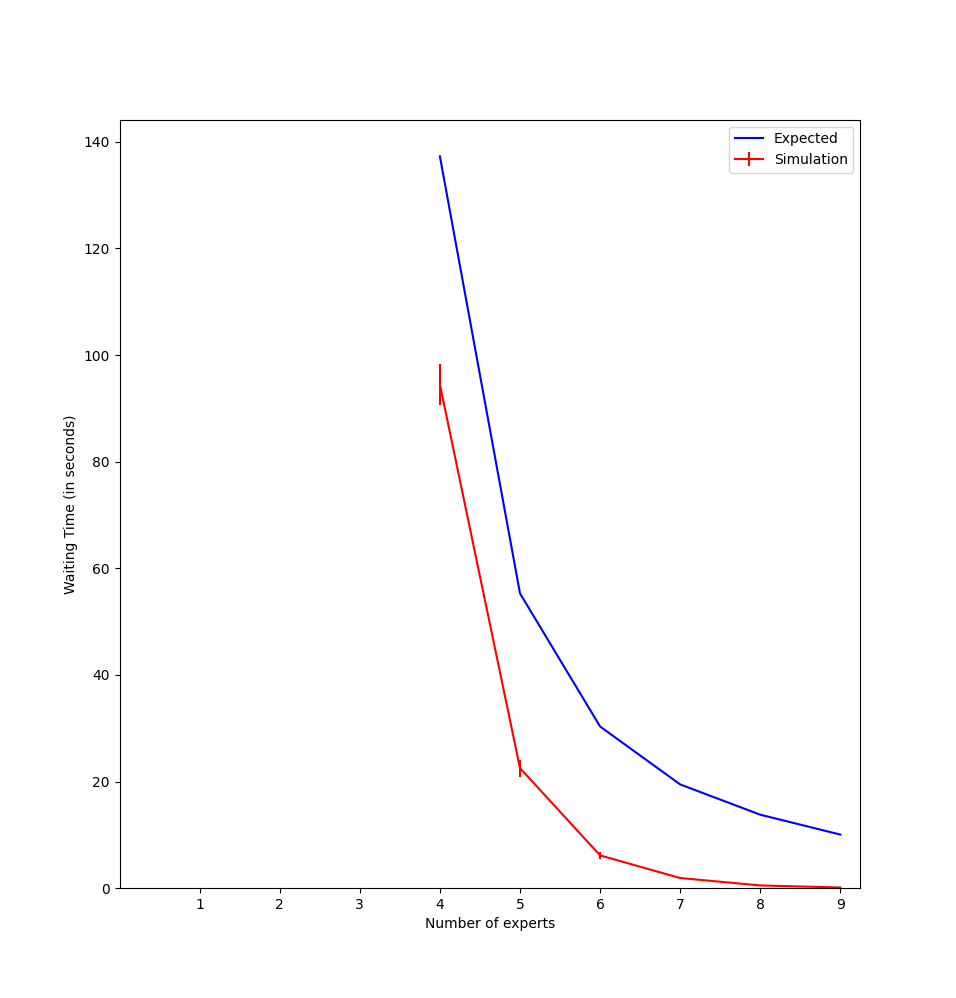
\includegraphics{figures/montecarlo/independent_calls_expon.png}
  \caption[
  The waiting times resulting from Simulation 1 and Formula~\ref{eq:mmn}
  ]{
    The waiting times resulting from Simulation 1 and Formula~\ref{eq:mmn}.
    The time values were sampled from the distributions shown in
    Figure~\ref{fig:simple_sim1_dists}.
    The number of users in the system varies as described in
    Section~\ref{sec:simple}.
  }\label{fig:simple_sim1_results}
\end{figure}

\begin{table}
  \begin{tabular}{|l|l|}
    \hline
    \textbf{Inter-Arrival Times} & \\
    \hline
    Distribution Type & Exponential\\
    \hline
    $\lambda$ & 1 / 60 seconds\\
    \hline
    \hline
    \textbf{Service Times} & \\
    \hline
    Distribution Type & Exponential\\
    \hline
    $\lambda$ & 1 / 180 seconds\\
    \hline
  \end{tabular}
  \caption{
    Parameter values for the distributions that Simulation 1 samples from
  }\label{tab:sim1_params}
\end{table}

The \emph{system occupancy}, which is computed according to
Formula~\ref{eq:occupancy}, cannot exceed 1.
Otherwise, calls will arrive faster than they can be answered, and the queue
will continue to grow the longer the simulation is run.
We thus only report results for cases where the system occupancy is below 1.

\begin{equation}
\rho = \frac{\lambda}{N \mu}
\label{eq:occupancy}
\end{equation}

The number of users in the system at any given time was not fixed.
Instead, it is a function of the arrival process, service times, and the amount
of time users spend waiting in the queue.
Increasing the number of experts while leaving all other parameters the same
will decrease time spent in the queue, which will reduce the number of users in
the system overall.

\subsection{Lognormal Service Times}\label{sec:sim_lognormal}

Service times are exponentially distributed in the M/M/N model.
However, two studies of logs from actual call centers have shown service times
to be lognormally distributed~\cite{queue1, queue2}.
A normal distribution follows a bell curve, with mean $\mu$ and standard
deviation $\sigma$.
If $\ln{(X)}$ follows a normal distribution, this means that $X$ is lognormally
distributed.
Figure~\ref{fig:simple_sim2_dists} shows an example of a probability density
function for a lognormal distribution.

\begin{figure}[h]
  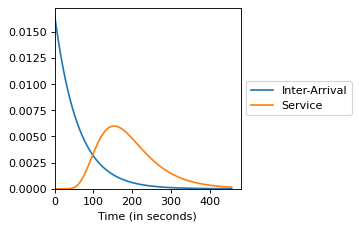
\includegraphics{figures/montecarlo/expon_lognorm.png}
  \caption[The PDFs for the distributions that Simulation 2 samples from]{
    The PDFs for the distributions that Simulation 2 samples from.
    The inter-arrival times were sampled from an exponential distribution.
    The service times were sampled from a lognormal distribution.
  }\label{fig:simple_sim2_dists}
\end{figure}

The probability density function for a lognormal distribution is:
\[
  \frac{1}{x \sigma \sqrt{2 \pi}}
  \exp{\left( - \frac{\left( \ln(x) - \mu \right)^2}{2 \sigma^2} \right)}
\]

Lognormal service times require an M/G/N model, which has a Poisson arrival
process, more than one server, and allows for any distribution of service times.
\citet{queue1} examined the expected call center wait time using
Formula~\ref{eq:mgn}, which is an approximation of an M/G/N queue.

\begin{equation}
  E[\text{Wait for M/G/N}] \approx E[\text{Wait for M/M/N}] *
  \frac{1 + (\sigma_s * \mu)^2}{2}
\label{eq:mgn}
\end{equation}

$E[\text{Wait for M/M/N}]$ is computed according to
Formula~\ref{eq:num_waiting}.
$\sigma_s$ is the standard deviation of service times.
$\mu$ is the average service rate.
Note that the average service time is $1/\mu$.

\subsubsection{Simulation 2}

We modified Simulation 1 to sample service times from a lognormal
distribution, but we kept the exponential distribution for inter-arrival time
samples.
We will refer to this version of the simulation as Simulation 2.
The distributions for Simulation 2 are depicted in
Figure~\ref{fig:simple_sim2_dists}, and the parameters of these distributions
are listed in Table~\ref{tab:sim2_params}.
The results from the simulation and Formula~\ref{eq:mgn} are shown in
Figure~\ref{fig:simple_sim2_results}.
The average arrival rate and average service rate for Formula~\ref{eq:mgn} were
computed based on the inter-arrival times and service times that were sampled by
the simulation.
The waiting times from the simulation were slightly higher than the waiting
times from the formula in every case.
We believe this difference is due to the fact that Formula~\ref{eq:mgn} is just
an approximation.
In addition, the formula is approximating a queue with an arbitrary probability
distribution for service times.
Thus it is more general than our simulation, which specifically uses a lognormal
distribution for service times.

\begin{table}
  \begin{tabular}{|l|l|}
    \hline
    \textbf{Inter-Arrival Times} & \\
    \hline
    Distribution Type & Exponential\\
    \hline
    $\lambda$ & 1 / 60 seconds\\
    \hline
    \hline
    \textbf{Service Times} & \\
    \hline
    Distribution Type & Lognormal\\
    \hline
    $\sigma$ & 0.4 log(seconds)\\
    \hline
    $\mu$ & log(180 seconds)\\
    \hline
  \end{tabular}
  \caption{
    Parameter values for the distributions that Simulation 2 samples from
  }\label{tab:sim2_params}
\end{table}

\begin{figure}[h]
  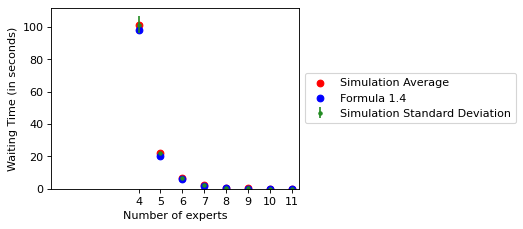
\includegraphics{figures/montecarlo/independent_calls_lognorm.png}
  \caption[
  The waiting times resulting from Simulation 2 and Formula~\ref{eq:mgn}
  ]{
    The waiting times resulting from Simulation 2 and Formula~\ref{eq:mgn}.
    The time values were sampled from the distributions shown in
    Figure~\ref{fig:simple_sim2_dists}.
    The system occupancy was greater than 1 when there were fewer than 4
    experts, so we do not have results for these cases for the reasons that we
    describe in Section~\ref{sec:simple}.
    The number of users in the system varies as described in
    Section~\ref{sec:simple}.
  }\label{fig:simple_sim2_results}
\end{figure}

\subsection{Simulating All Steps}

We expanded our simulation to model users completing an entire task with a WCA
application.
We will refer to this version as Simulation 3.
Rather than starting at the point that a call comes into the call center, we
also model users receiving automated guidance and calling for help if they get
stuck.
The simulation includes user patience, which is the amount of time a person is
willing to spend on a step, before they give up and call the expert.
Most steps of the task will be feasible.
This means that a user will eventually complete the step if they spend enough
time on it.
However, a user's patience is finite.
In addition, some steps might be infeasible, which means that the user cannot
complete them without calling the expert.
Infeasible steps could be a result of incorrectly manufactured parts, bad
lighting, or poorly trained machine learning models.
It is therefore in the user's best interest to give up on a step and call the
expert at some point.

Simulation 3 models users from the point they begin the task.
We will refer to the time that the user starts the task as the
\emph{entrance time}.
The amounts of time in between sequential entrance times (which we will
henceforth call inter-entrance times) are sampled from an exponential
distribution.
The number of users completing the task at any given point is a function of the
arrival process, and the lengths of time that it takes users to complete the
full task.
The simulation models users completing the task according to the process
described in Algorithm~\ref{algo:sim}.
This process is repeated for each simulated user.
The simulation allows users to work in parallel.
However, if a user calls for help while all experts are busy, they must wait in
a queue for service.
As in the previous simulations, all users wait in a single queue that is
serviced in FIFO order.

\begin{algorithm}[H]
  \For{step in task}{
    sample patience length\;
    sample step feasibility\;
    \eIf{\text{step feasibility is 1}}{
      sample step length\;
      \eIf{\text{step length < patience length}}{
        Pause for step length\;
        User completes step successfully\;
      }{
        Pause for patience length\;
        User calls expert for help\;
        }
      }{
        Pause for patience length\;
        User calls expert for help\;
    }
  }
  \caption{
    The process simulating one user completing a task using a WCA application
  }\label{algo:sim}
\end{algorithm}

Simulation 3 samples from distributions used in existing literature.
Patience length is sampled from a generalized Pareto distribution.
Probability theory considers patience lengths to be extreme
values~\cite{patience}.
A generalized Pareto distribution can be used to model extreme values.
The generalized Pareto distribution has parameters for location ($\mu$), scale
($\sigma$), and shape ($\xi$).
$\mu$ is equivalent to the mode of a generalized Pareto distribution, rather than
the mean.
$\sigma$ is not the standard deviation of a generalized Pareto distribution.
The probability density function of a generalized Pareto distribution is:
\[
  \frac{1}{\sigma} \left(1 + \left(\xi * \frac{x - \mu}{\sigma}\right)
  \right)^{-(1/(\xi + 1))}
\]


\citet{patience} found a generalized Pareto distribution to be a good fit for
samples of time that people waited before crossing streets, while the crossing
signal was telling them not to cross.

Step feasibility was sampled from a Bernoulli distribution.
A Bernoulli distribution models events with two possible outcomes.
It uses a single parameter $p$, which is the probability of one outcome.
Probability values must sum up to one, so the probability of the other outcome
is $1-p$.

Step length was sampled from an exponentially modified Gaussian distribution.
An exponentially modified Gaussian random variable is the sum of an
exponentially distributed random variable and a normally distributed random
variable, that are both independent of each other.
\citet{dawson1988fitting} suggested modeling response times from an
exponentially modified Gaussian distribution.
Figure~\ref{fig:sim3_dists} shows the generalized Pareto and exponentially
modified Gaussian distributions that were used.

When the sampled step feasibility value is 1, and the patience length value is
smaller than the step length value, the user will call the expert for help.
This represents a user giving up on a step that is feasible.
One can increase the proportion of steps that a user will give up on by shifting
the step length distribution to the right and/or shifting the patience length
distribution to the left.

\begin{figure}[H]
  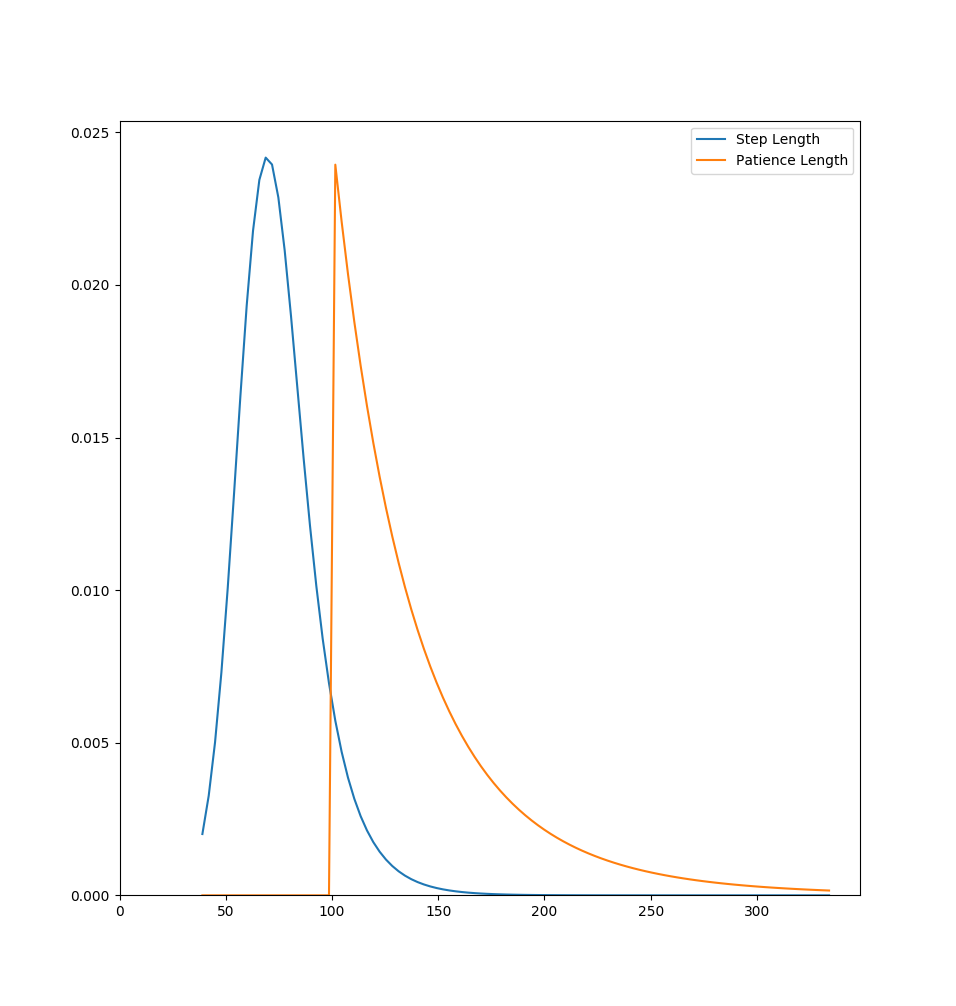
\includegraphics{figures/montecarlo/step_patience.png}
  \caption[The PDFs for the distributions that Simulation 3 samples from]{
    The PDFs for the distributions that Simulation 3 samples from.
    Patience length is sampled from a generalized Pareto distribution and step
    length is sampled from an exponentially modified Gaussian distribution.
    Sampling from these distributions resulted in users giving up on about 2.5\%
    of feasible steps.
  }\label{fig:sim3_dists}
\end{figure}

The samples from the exponential distribution that were used to determine
Inter-entrance times for users starting the task are shown in
Figure~\ref{fig:arrival_times}.
The times at which a user in our simulation called for help are shown in
Figure~\ref{fig:step_patience}.
We fit an exponential curve to both of these sets of data.
The $R^2$ for the exponential fit was 0.99 for the inter-entrance times.
This strong exponential fit is expected, because these times were drawn from an
exponential distribution.
The exponential fit for the inter-arrival times of users calling for help had
an $R^2$ of 0.983.
This indicates that Simulation 2, which simply models calls coming in with
exponential inter-arrival times, might be accurate enough for modeling call
centers for WCA applications.

\begin{figure}[H]
  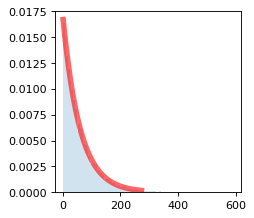
\includegraphics{figures/montecarlo/arrival_times.png}
  \caption[Inter-entrance time samples from Simulation 3]{
    Inter-entrance time samples from Simulation 3.
    The inter-entrance time samples for users starting the task are shown in
    blue.
    These were drawn from an exponential distribution.
    We fit an exponential curve to this data, which is shown in red.
  }\label{fig:arrival_times}
\end{figure}

\begin{figure}[H]
  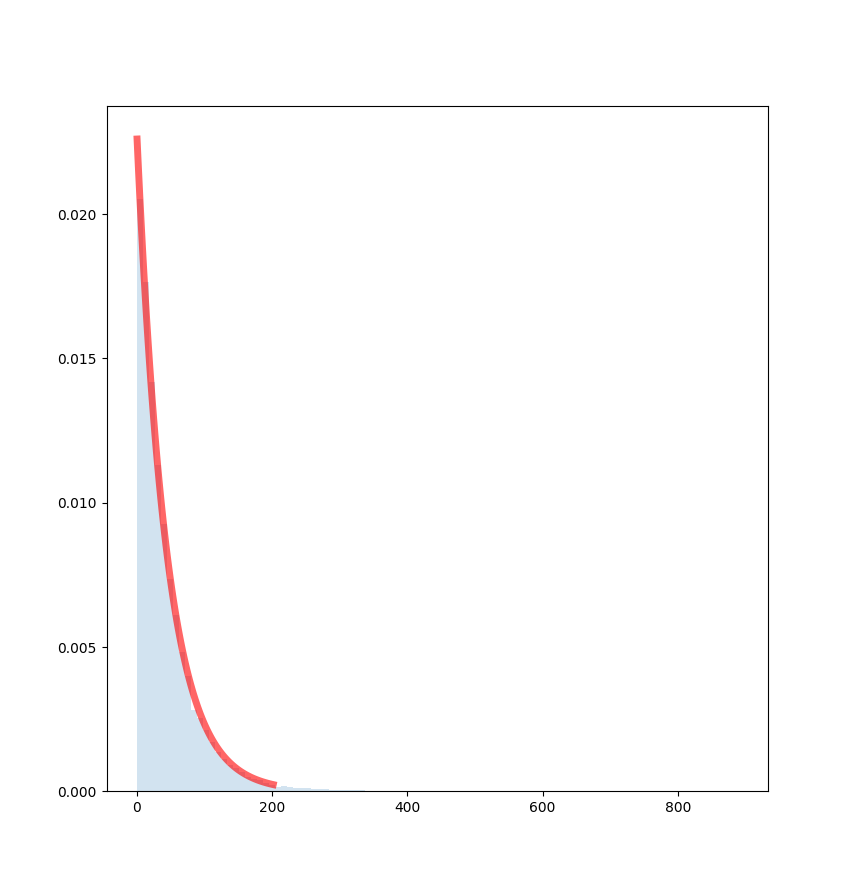
\includegraphics{figures/montecarlo/call_times.png}
  \caption[Inter-arrival times for help calls that resulted from Simulation 3]{
    Inter-arrival times for help calls that resulted from Simulation 3.
    We fit an exponential curve to this data, which is shown in red.
  }\label{fig:step_patience}
\end{figure}

\subsubsection{Servicing Calls}

Our simulation sampled service times from a lognormal distribution.
All of the parameters for the distributions sampled from in Simulation 3 are
shown in Table~\ref{tab:sim3_params}.
The average waiting time for users in our simulation is shown in
Figure~\ref{fig:full_expected_sim}, along with the expected waiting times from
Formula~\ref{eq:mgn}.
There was a huge variation in waiting time across different runs of the
simulation with five experts.
However, this variation decreased substantially when we ran the simulation with
six experts.
This makes sense intuitively, as there was more of a buffer to handle bursts of
calls coming in.

\begin{table}
  \begin{tabular}{|l|l|}
    \hline
    \textbf{Step Lengths} & \\
    \hline
    Distribution Type & Exponentially modified Gaussian\\
    \hline
    $\mu$ & 60 seconds\\
    \hline
    $\sigma$ & 12 seconds\\
    \hline
    $\lambda$ & 1 / 15 seconds\\
    \hline
    \hline
    \textbf{Patience} & \\
    \hline
    Distribution Type & Generalized Pareto\\
    \hline
    $\mu$ & 100 seconds\\
    \hline
    $\sigma$ & 40 seconds\\
    \hline
    $\xi$ & 0.1\\
    \hline
    \hline
    \textbf{Step Success} & \\
    \hline
    Distribution Type & Bernoulli\\
    \hline
    $p$ & 0.95\\
    \hline
    \hline
    \textbf{Inter-Arrival Times} & \\
    \hline
    Distribution Type & Exponential\\
    \hline
    $\lambda$ & 1 / 60 seconds\\
    \hline
    \hline
    \textbf{Service Times} & \\
    \hline
    Distribution Type & Lognormal\\
    \hline
    $\sigma$ & 0.4 log(seconds)\\
    \hline
    $\mu$ & log(180 seconds)\\
    \hline
  \end{tabular}
  \caption{
    Parameter values for the distributions that Simulation 3 samples from
  }\label{tab:sim3_params}
\end{table}

\begin{figure}[h]
  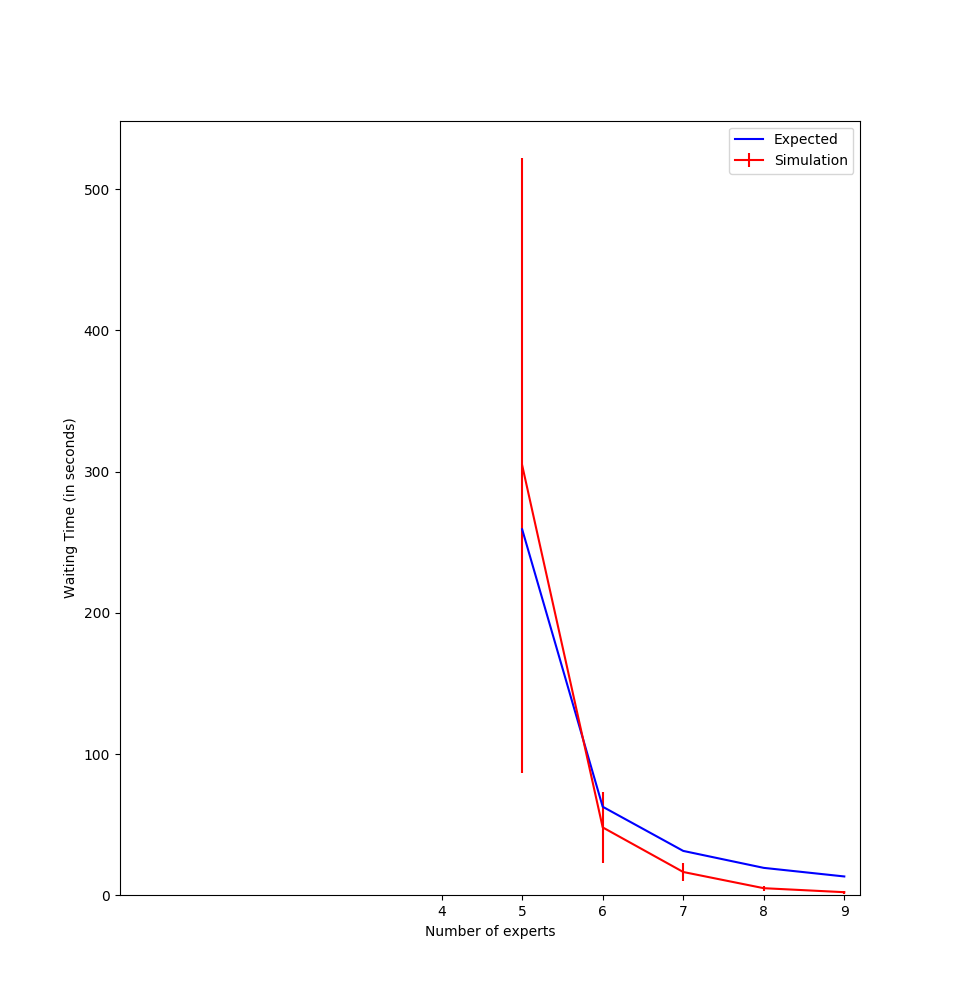
\includegraphics{figures/montecarlo/full_expected_sim.png}
  \caption[Waiting times from Simulation 3 and Formula~\ref{eq:mgn}]{
    Waiting times from Simulation 3 and Formula~\ref{eq:mgn}.
    The standard deviation of waiting times from the simulation was large when
    there were five experts.
    However, increasing the number of experts decreased this standard deviation.
    The number of users in the system varies as described in
    Section~\ref{sec:simple}.
  }\label{fig:full_expected_sim}
\end{figure}

The simulation results are plotted against the times from Formula~\ref{eq:mgn}
in Figure~\ref{fig:gof}.
Fitting a linear model to these values achieves an $R^2$ coefficient of 0.86.
This fit indicates that the waiting times from the simulation are reasonably
well correlated with the waiting times from the formula.

\begin{figure}[H]
  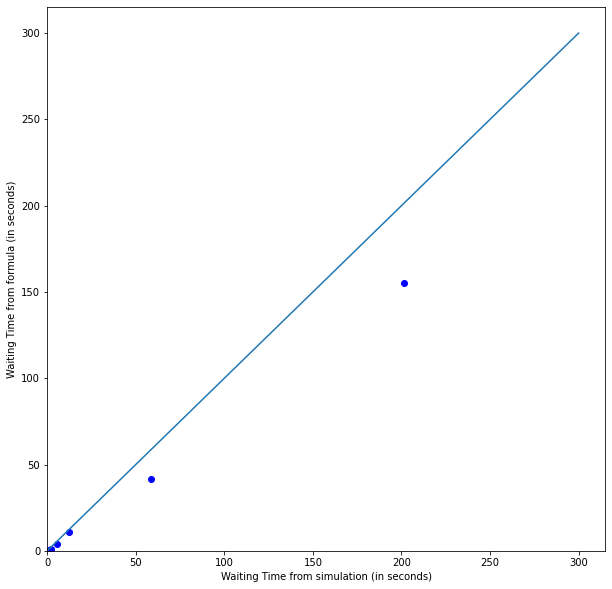
\includegraphics[width=0.5\textwidth]{figures/montecarlo/gof.png}
  \caption[
  Waiting times from Simulation 3 plotted against times from
  Formula~\ref{eq:mgn}
  ]{
    Waiting times from Simulation 3 plotted against times from
    Formula~\ref{eq:mgn}.
    The waiting times in Figure~\ref{fig:full_expected_sim} drop significantly
    when the number of experts is increased from 5 to 6.
    Thus there is a large gap between the points in this figure.
  }\label{fig:gof}
\end{figure}

\section{Open Source Tool}

We did not have data for real workers completing WCA tasks and calling experts
for help.
We therefore chose parameter values for the distributions that our simulations
sampled from based on our experiences developing and using WCA applications.
In order to make our work helpful for a practitioner staffing a call center for
a real WCA application, we developed a tool that runs our simulations based on
real data for a specific WCA application.
In order to use this tool, a user inputs data samples collected from a call
center.
The required samples are lengths of task steps, lengths of user patience,
lengths of calls, inter-entrance times of workers, and the probability of a user
completing a step correctly.

The tool is available as a Google Colab notebook.
Google Colab is a web based service for running Python code.
A Colab notebook can also be downloaded and run locally as a Python script or a
Jupyter notebook.
We have posted the tool
publicly\footnote{\url{https://cmusatyalab.github.io/roger-thesis/}} under
Version 2.0 of the Apache License.
All of the source code is available at that link.
There is a version of the tool that allows users to copy and paste data samples
into a web form, and a second version that allows users to upload data as CSV
files.
After a user uploads data, the notebook fits distributions to this data and
runs the simulation with samples from the newly-fitted distributions.
The notebook generates a graph similar to Figure~\ref{fig:full_expected_sim}.

\section{Exploring Parameter Space}

This simulation allows us to see how average wait time changes, when we modify
one variable and leave all other variables constant.
Although the quantitative outcomes will depend on the specific source
distributions, which were parameterized here based on observation of previous
WCA applications, the results of these simulations illustrate the pronounced
increases in wait time that occur given a shift in critical parameters, such as
greater incidence of infeasible steps, reduced user patience, or inclusion of
more long steps that lead users to call on the expert.

We ran these simulations with nine experts.
We sample from the same distributions used in Simulation 3.
The simulation was run ten times for each variable value we tested.

\subsection{Varying the Proportion of Feasible Steps}\label{sec:feasible}

This experiment varied the proportion of steps that a user could complete.
A feasible step is one that a user can complete if they spend enough time on it.
However, a user might choose to give up and call the expert before the step is
complete.
Users are guaranteed to complete a feasible step if they spend enough time on
it.
However, the user might actually give up and call the expert before they have
spent the time necessary to complete the step.
An infeasible step cannot be completed unless the user calls the expert.
Results are shown in Figure~\ref{fig:vary_success}.
As the proportion of infeasible steps increases, the average waiting time
increases.
This is because an increase in the number of infeasible steps will increase the
number of calls to the expert.

\begin{figure}[h]
  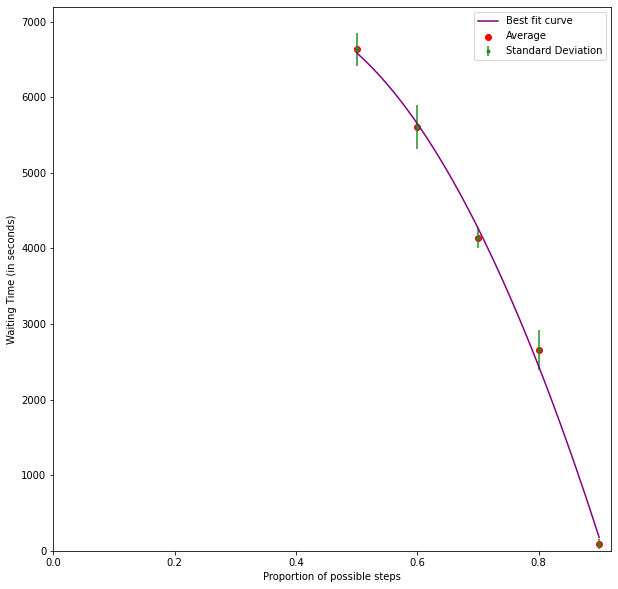
\includegraphics{figures/montecarlo/vary_success.png}
  \caption[
  Average wait times resulting from changing the proportion of feasible steps
  ]{
    Average wait times resulting from changing the proportion of feasible steps.
    These wait times were fit by a second-order polynomial as shown, with an
    $R^2$ value of over 0.99.
    This indicates a steep cost as a WCA application is penetrated by infeasible
    steps, for example, due to ineffective image processing or manufacturing
    error.
    As we describe in Section~\ref{sec:feasible}, feasible steps are those that
    are completable, but a user may still give up on a feasible step and call
    the expert.
  }\label{fig:vary_success}
\end{figure}

\subsection{Varying Patience Length}

Patience length is the amount of time that a user is willing to spend trying to
complete a step, before calling the expert.
The average waiting time that resulted from different average lengths of
patience are shown in Figure~\ref{fig:vary_patience}.
Increasing average patience length will increase the number of steps that users
will complete on their own without calling the expert.
The number of calls to experts therefore decreases.
Thus the average waiting time decreases as average patience length increases.

\begin{figure}[h]
  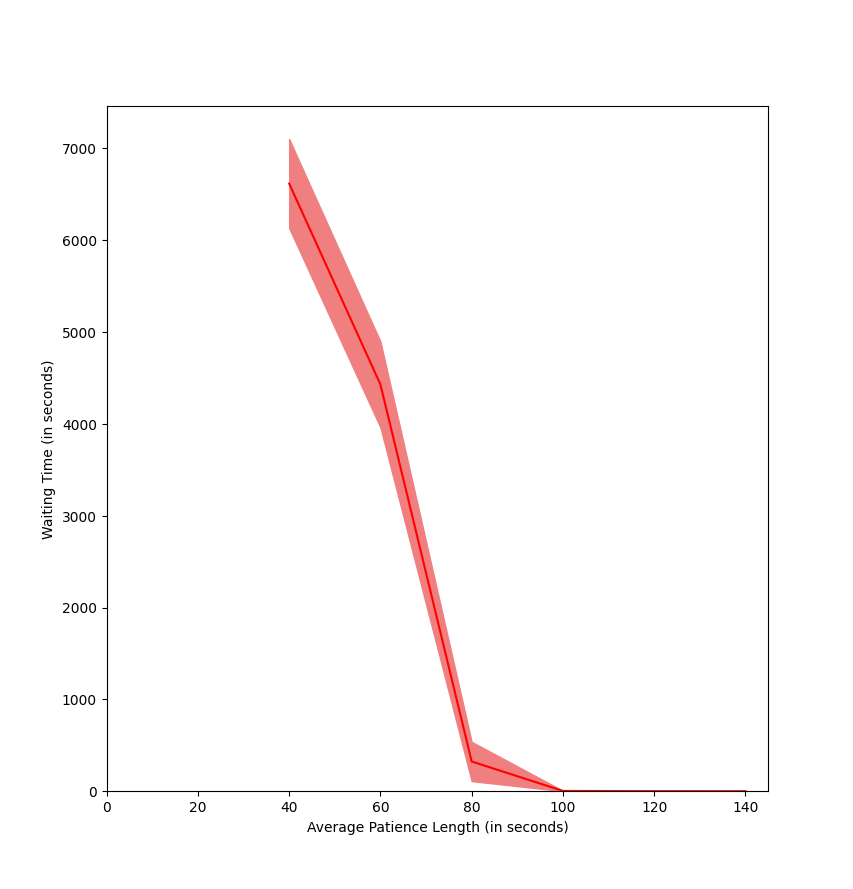
\includegraphics{figures/montecarlo/vary_patience.png}
  \caption[
  Average wait times resulting from changing users' simulated patience
  ]{
    Average wait times resulting from changing users' simulated patience.
    Given the current parameters, with nine experts available, the waiting times
    move from a scale of minutes to hours when the patience length is doubled
    from 40 sec to 80 sec.
    A Generalized Pareto distribution, which is what we use to sample patience
    lengths, is parameterized by its mode.
    This is thus the parameter that we vary, in order to change patience length
    samples.
  }\label{fig:vary_patience}
\end{figure}

\subsection{Varying Length of Feasible Steps}

This experiment varied the average amount of time that a user must spend in
order to complete a feasible step.
Figure~\ref{fig:vary_step_length} shows the results of this.
Increasing average step length increases the likelihood that a step will take
longer than a user's patience length.
This results in more calls being made to the expert.
Therefore, increasing average step length increases the average waiting time.

\begin{figure}[H]
  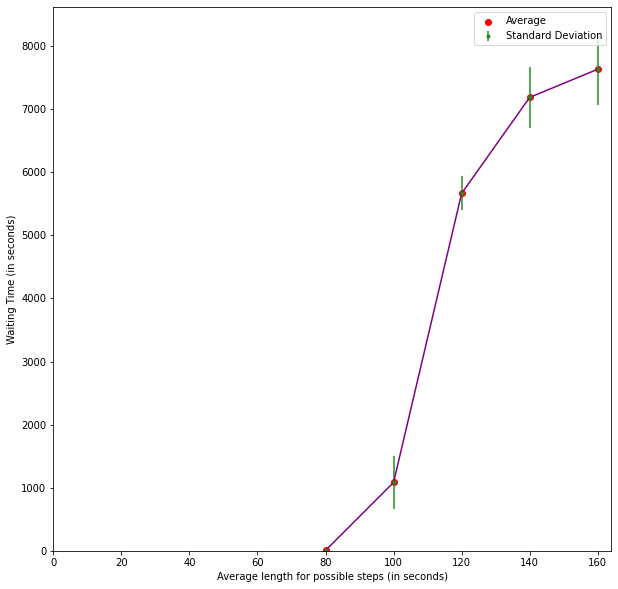
\includegraphics{figures/montecarlo/vary_step_length.png}
  \caption[Average wait times resulting from changing the average step length]{
    Average wait times resulting from changing the average step length.
    Step length refers to the amount of time it took to complete a step that was
    feasible.
    See Section~\ref{sec:feasible} for how we define a feasible step.
    Given the current parameters, with nine experts available, doubling the
    average
    step length from 80 sec to 160 sec moved waiting times from essentially no
    waiting to over 2 hours.
  }\label{fig:vary_step_length}
\end{figure}

\section{Limiting the Number of Active Users}

WCA applications might be licensed for use by a certain number of people at
any given time.
We will henceforth use the term ``active users'' to refer to the number of
people using an application at a given time.
For example, an organization might buy a license for a WCA application that
supports 10 active users.
If 10 people from this organization are using the application, and an 11th
person tries to start using it, the 11th person will be given an error message
saying that the organization only paid for a license for 10 active users.
This error message will prevent the application from starting.

This licensing strategy has the advantage of limiting the resources required to
support application users.
The licenses could be specific to a particular location.
In this case, a provider could provision cloudlet resources at that location in
order to support the number of active users that a license allows.
In addition, limits on the number of active users make it easier to decide how
many human experts to have available in the call center.

We created a version of our simulation that included a limit on the number of
active users.
We will henceforth call this version Simulation 4.
Simulation 4 is identical to Simulation 3 while the number of active users is
below the limit.
Once the number of active users reaches the limit, new users will be unable to
start the task.
One of the active users must complete the task, which will cause the number of
active users to drop below the limit, before a new user will be allowed to begin
the task.
Users attempt to begin the task according to the same Poisson arrival process
used in Simulation 3.
However, if a user attempts to begin the task while the number of active users
is equal to the limit, they will leave the simulation without starting the task.

Figure~\ref{fig:vary_num_users} shows the average waiting times that resulted
from running Simulation 4 with different limits on the number of users.
Figure~\ref{fig:vary_num_users2} shows the number of experts that were required
to achieve certain average wait times for users in the queue.

\begin{figure}[h]
  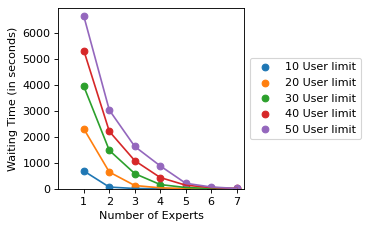
\includegraphics{figures/montecarlo/vary_num_users.png}
  \caption[Average wait times resulting from Simulation 4]{
    Average wait times resulting from Simulation 4.
    We varied the number of experts and the limit on the number of active users
    allowed in the simulation.
  }\label{fig:vary_num_users}
\end{figure}

\begin{figure}[h]
  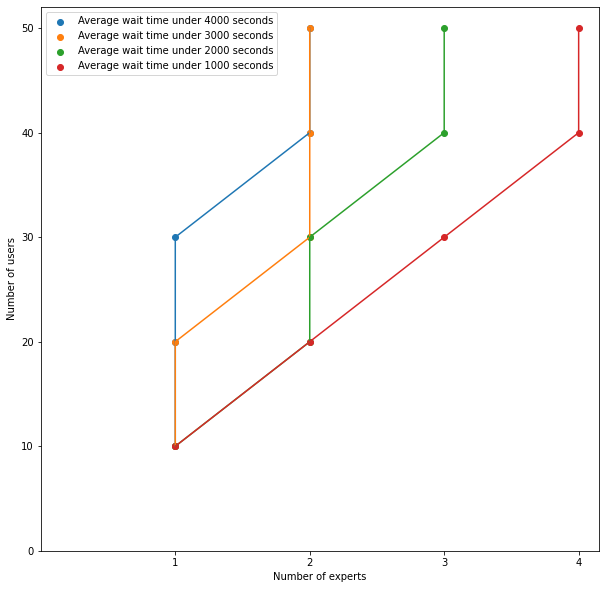
\includegraphics{figures/montecarlo/vary_num_users2.png}
  \caption[
  The number of users that were serviced under certain wait time thresholds
  ]{
    The number of users that were serviced under certain wait time thresholds.
    These numbers were obtained from Simulation 4.
    As expected, the number of users increased as we increased the number of
    experts.
  }\label{fig:vary_num_users2}
\end{figure}

\section{Summary}

In order to help users correct mistakes that they make completing an assembly
task with the help of a WCA application, we added a call functionality to our
applications.
Users can press a button to request help from a task expert, who can see the
user's camera feed and talk back and forth with the user.
We developed and evaluated Monte-Carlo based tools to predict the number of
experts that must be available to help a given set of users.
